\section{Model validation and extrapolation for Hamamatsu VUV4}
\label{sec:extrapolation}

The model is tested by extrapolating in wavelength and comparing with Hamamatsu reported vacuum PDE, and LXe measurements from literature. \autoref{fig:hpk_datasheet} shows the HPK reported PDE, the 4~V TRIUMF data and prediction at two temperatures. Beyond 500~nm, increasing the model temperature from 160~K to 273~K increases the PDE to approach the datasheet, giving confidence to the temperature dependence implementation above $\sim 500$~nm. Below 500~nm, the TRIUMF measurement and corresponding model extrapolation to the VUV is $\sim$2\% higher than the datasheet. Overall the model predicts the reported shape from 160-350~nm well. In the VUV, silicon quantum yield is applied to $P_e$ as outlined in \autoref{sec:internal_pde}\footnote{We approximate the quantum yield from \cite{Lewis_2025_qy} as $\eta(\lambda) = (\frac{300~\text{nm}}{\lambda})^{3/2}$}. Extrapolation to wavelengths relevant for ExCT are shown in inset of \autoref{fig:hpk_wlen_fit}.

%%%%%
\begin{figure}[h]
\centering
% \includegraphics[width=.9\linewidth]{fig-t_datasheet_comp.png}
% 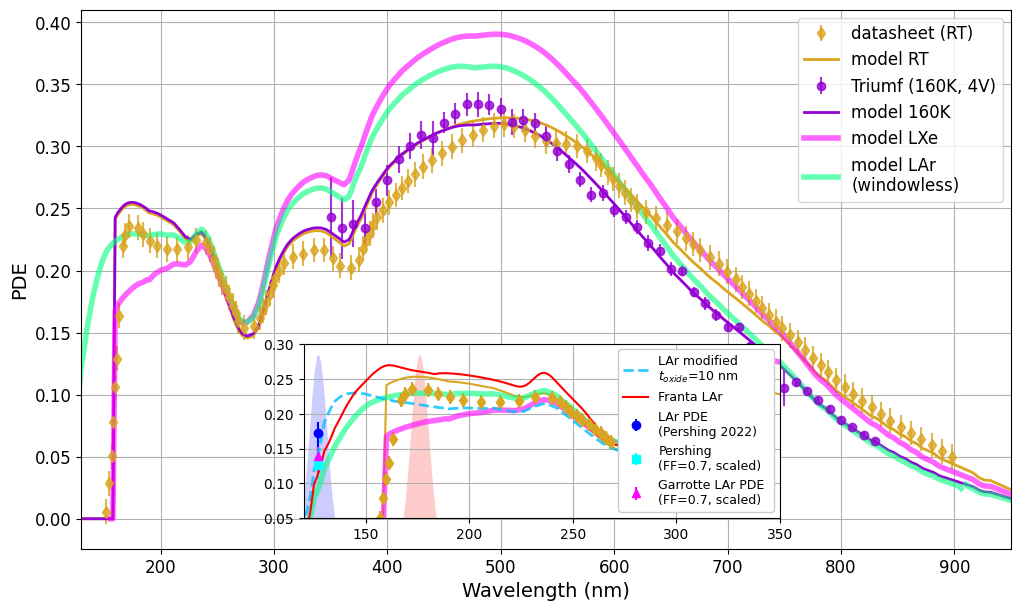
\includegraphics[width=.9\linewidth]{fig-datasheet_simplified.png}
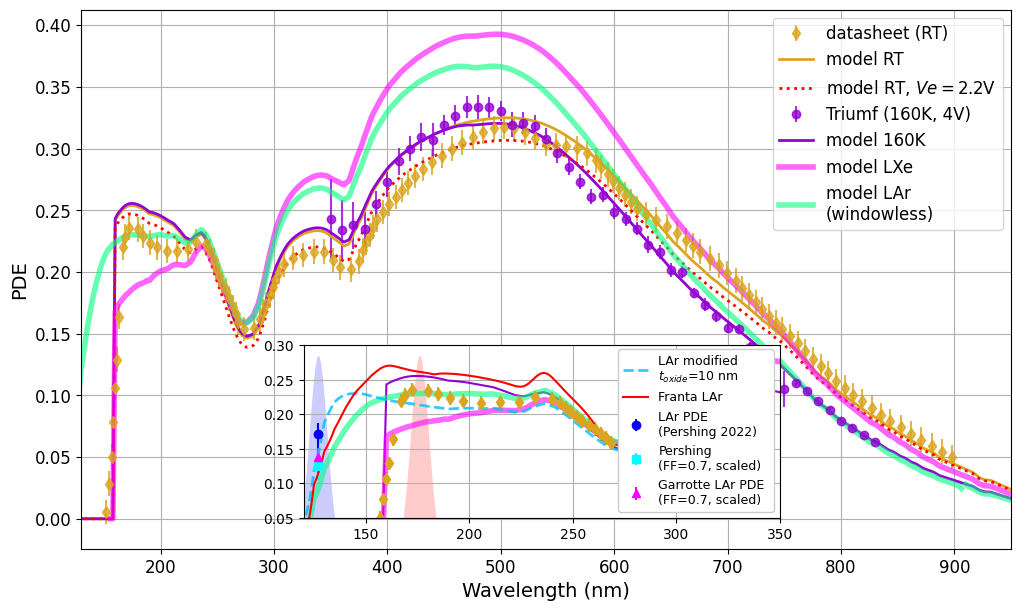
\includegraphics[width=.8\linewidth]{fig-datasheet_simplified_lowerPe.png}
\caption{\label{fig:hpk_datasheet}
Comparison of the HPK reported PDE (at room temperature - RT), measured PDE (TRIUMF cold) and the PDE model for different inputs. Increasing the model's temperature from 160~K to 273~K improves the Vis-NIR prediction compared to the datasheet. Thicker lines are the estimated PDE in LXe, and LAr without quartz window. Inset shows the VUV region in detail, including the Franta result (higher due to shalower $dp^*$ driven by curvature in $n, k$ data) and a second LAr prediction with a thinner oxide. The red dotted line is model with reduced $P_e$ ($V_e=2.2$~V), in better agreement with datasheet. The LAr datapoints are from \cite{Pershing_2022_argonPDE, garrote_2024_cryoPDE}, scaled by the $FF$ of each device.}
\end{figure}
%%%%%

The differences between data may be due to measurement systematics or temperature differences. More likely is device-to-device variation due to manufacturing and handling, which is difficult to account for analytically. We take this extrapolation as evidence for the predictive power of the model, showing VUV efficiency can be predicted using UV/IR efficiency, quantum yield, and VUV reflectivity to constrain oxide thickness.

The predicted LAr and LXe PDE show an increase in the visible region due to improved optical coupling. For LXe the transmission decreases below 250~nm as $n_{LXe} \approx n_{\sio} < n_{\si}$ and the enhancement from constructive interference is reduced. Reduction of UV LXe efficiency is consistent with other preliminary measurements \cite{Alex_2024LoLX2}. For the 175~nm centered xenon emission, the maximum achievable transmission in liquid is $\sim40\%$ with $\tox = 44$~nm. The VUV4's $\tox$ yields $\sim$55\% vacuum transmission and 38\% in liquid; the $\sim$17~nm oxide is well optimized LXe scintillation in gas or liquid. For FBK the average thickness yields transmission of 38\% in vacuum and 39\% in liquid, similar to the ray-optics values as oscillations are averaged over the emission spectrum.

The falloff in the PDE at 160~nm is due to absorption on the quartz window. In \cite{Pershing_2022_argonPDE} the window is removed and PDE for LAr scintillation of $\sim 14–17\%$ is reported for two VUV4 devices. Dividing by fill factor and assuming $iPDE=1$, the reported efficiencies require transmissions between $20-28\%$ at 127~nm. Our optical model cannot produce transmission this high, giving $T(128\text{nm})=17.0^{+1.4}_{-1.2}\% $ for the default dataset and $T(128\text{nm})=20.7^{+1.2}_{-0.6}\%$ with Franta. Within the constraints of our model, a combination of thinner oxide and reduced $k_{\sio}$ is required to achieve transmissions approaching 28\%. Perfect internal efficiency would be driven by an increase in charge collection efficiency (reduced $dp^*$) \cite{cce_cryogenic_1998, biroth_2015_cryogenic} or higher $P_e$ due to lower temperature.
% For example scaling $k_{\sio}$ by 50\% and reducing $\tox$ by 5, 3~nm yields 28\% transmission for default, Franta datasets respectively. 

\begin{figure}[htbp]
\centering
% \includegraphics[width=0.9\linewidth]{fig-VUV4_reflectivity_validation_2_onlyData.png}
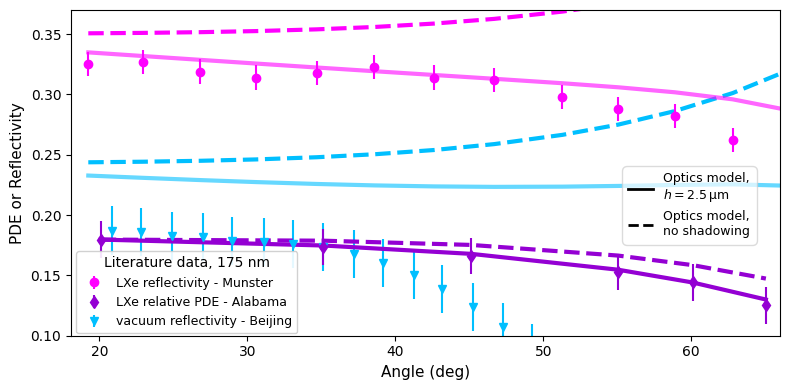
\includegraphics[width=0.8\linewidth]{fig-VUV4_reflectivity_validation_dataOnly_wider.png}
\caption{Optical model compared to angular responses for VUV4 device for $175$~nm light or LXe emission. Solid lines show optical model including shadowing, the dashed lines without shadowing. Relative PDE data (Alabama, \cite{Nakarmi_2020}) is scaled vertically to compare with the model. In all cases shadowing better describes the data. Vacuum data (Beijing, \cite{sipmRef_nexo_guofu}) is lower than expectation from $R_{SiPM} = FF \cdot R_{\si}$, but predicted LXe reflectivity agree (Munster, \cite{Wagenpfeil_2021}).\label{fig:vuv4_reflectivity}.}
\end{figure}

In \autoref{fig:vuv4_reflectivity} we compare the model's angular predictions with shadowing to LXe measurements of reflectivity \cite{Wagenpfeil_2021} and relative PDE \cite{Nakarmi_2020}. Vacuum reflectivity from \cite{sipmRef_nexo_guofu} is also included showing the reduction relative to the assumption
$R(\theta){\mathrm{SiPM}} = FF(\theta)\cdot R{\mathrm{Si}}$. Our model predicts the absolute LXe reflectivity well (upper pink data and dashed line), and shadowing is clearly required to reproduce the monotonic decrease in reflectivity and best describes the relative PDE. 